\chapter{Photonic Qubit Path} \label{chapter:photonic_qubit_path}

This chapter describes the optical beam path used to deliver photonic qubits to the atom-cavity system and analyze them after reflection. The central challenge is that the birefringent cavity introduces a polarization-dependent amplitude mismatch of the reflected field requiring external compensation to achieve the optimal CNOT gate overlap.

\section{Polarization-Dependent Losses}\label{section:polarization_dependent_losses}

The reflection amplitude of a photon incident on an atom-cavity system, given by equation \eqref{eq:analytical_reflection}, depends sensitively on the system parameters: the coupling strength $g$, the cavity decay rate of the photons $\kappa$, the cavity outcoupling ratio $\kappa_{OC}$, the mode-matching between the fiber mode and the incoupling mirror surface $\mu_{fr}$, the mode matching between the fiber mode and the cavity mode $\mu_{fc}$, and the birefringence of the cavity $\Delta_{\text{biref}}=2\pi\cdot 500\text{MHz}$. Looking at the reflection scheme for \eqref{eq:reflection_cnot} in the basis defined in \eqref{eq:cnot_basis}, it becomes apparent that in order to achieve the highest possible overlap with an ideal CNOT gate, the reflection amplitudes $|r_{\pi}|$ and $|r_{V}|$, must (ideally) be the same. However, for the cavity parameters realized in this system (characterized in section \ref{section:experimental_parameters_for_gate}), this condition is not fulfilled.

As mentioned before, the $V$ mode of the birefringent cavity is detuned by $\Delta_{\text{biref}}=2\pi\cdot 500\text{MHz}$ from the $\pi$-mode, to which the atomic transition is resonantly coupled. This leads to a $V$ polarized photon, getting reflected from the first OC mirror without entering the cavity due to being far off-resonant. This then leads to the $V$ polarized component of both the CNOT input basis states, having a much larger relative reflection amplitude when compared to the $\pi$ polarized portion.

A $\pi$-polarized photon, on the other hand, interacts with the atom inside the cavity, making the reflection amplitude dependent on the atomic state. In the coupled case $\ket{1}$, the vacuum Rabi splitting shifts the dressed-state resonances to approximately $\omega_c\pm g$. This then leads to the photon being reflected off the OC mirror, but not perfectly, due to finite cooperativity. In the uncoupled state $\ket{0}$, the $\pi$-polarized photon fully enters the cavity, undergoes many round trips, and transmits back out teh OC mirror with a relative phase shift of $\pi$ compared to teh input field, on a timescale set by $1/\kappa_{OC}$. But due to intracavity losses (absorption, HR mirror leakage, imperfect mode-matching), the reflection amplitude is smaller than that of the coupled case.

Using the time-domain simulation described in Appendix \ref{appendix:qutip_simulation} with the parameters characterized in section \ref{section:experimental_parameters_for_gate}, the following reflection amplitudes are obtained:

\begin{table}[ht]
	\centering
	\begin{tabular}{l|c|c|c|c}
		\hline\hline
		             & $\ket{0,\pi}$   & $\ket{1,\pi}$  & $\ket{0,V}$    & $\ket{1,V}$    \\
		\hline
		$r$          & $-0.256+0.000i$ & $0.704+0.031i$ & $0.974+0.071i$ & $0.973+0.050i$ \\[6pt]
		$R = |r|^2$  & $0.064$         & $0.493$        & $0.953$        & $0.948$        \\[6pt]
		$\phi$ (rad) & $3.016$         & $0.000$        & $0.000$        & $0.000$        \\
		\hline
	\end{tabular}
    \caption{Reflection coefficients for the four input states of the atom-photon gate, simulated via a time-domain simulation outlined in Appendix \ref{appendix:qutip_simulation} using the system parameters characterized in section~\ref{section:experimental_parameters_for_gate}. The atomic states $\ket{0}$ and $\ket{1}$ correspond to the uncoupled and coupled ground states, respectively.}
	\label{tab:reflection_coefficients}
\end{table}

Table \ref{tab:reflection_coefficients} shows that the reflection amplitude for the $V$ polarized photon, is much bigger than that of the $\pi$ polarized photon, thus giving the following relationship: $|r_{V}| >|r_{\pi,\text{coupled}}| >|r_{\pi,\text{uncoupled}}|$.\\

This amplitude mismatch ultimately reduces the overlap with an ideal CNOT gate truth table. However, since the cavity parameters are fixed by the requirements of the broader \textit{CavityX} experiment, the atom-state-dependent amplitude difference cannot be addressed independently, as this would require changing the cavity itself. The following sections therefore focus on compensating the polarization-dependent mismatch, which can be corrected externally.


\section{Inducing Losses via a Brewster Window Array}

A Brewster window is a piece of uncoated UV fused silica. When placed at the so-called Brewster angle relative to the incoming light, then the p-polarized portion gets transmitted without any losses, while the s-polarized portion gets partially reflected. This effectively reduces the transmission through the optical element for s-polarized light. Here, the p-polarized light is identical to the $\pi$ polarized light, whereas the s-polarized light matches that of the $V$ polarized light.

As previously discussed in section \ref{section:polarization_dependent_losses}, in order to maximize the overlap of the measured CNOT gate truth table with that of an ideal CNOT gate, additional polarization-dependent losses must be included in the $V$ mode, to match those the $\pi$ mode experiences.

In order to achieve this an array of Brewster windows were installed on a custom machined mount, which place the Brewster windows at the Brewster angle relative to the incoming light, so that the $V$ polarized portion of the incoming light gets attenuated prior to interacting with the atom-cavity system. This ensures that in reflection, both polarization modes have the same reflection amplitude, allowing for the observation of the flip on the photonic qubit in the CNOT basis.

The Brewster angle can be simply calculated via:\cite{ThorlabsBW}

\begin{align}
	\tan{\theta_B}                                                 & = n_t/n_i                                                                                                 \\
	n_t^2 -1 = \frac{0.6961663 \lambda^2}{\lambda^2 - 0.0684043^2} & + \frac{0.4079426 \lambda^2}{\lambda^2 - 0.1162414^2} + \frac{0.8974794\lambda^2}{\lambda^2 - 9.896161^2}
	\label{eq:brewster_window_stuff}
\end{align}

In \eqref{eq:brewster_window_stuff} $n_t$ is the refractive index of the Brewster window, and $n_i$ would be the refractive index from which the incoming light is coming from (here: air $n_i \sim 1.004$). For light that is resonant to the 2-1' transition of the $\text{D}_2$-line of $^{87}\text{Rb}$, $n_t=1.453667$, resulting in a Brewster angle $\theta_B=55.467288^{\circ}$. Measurements outlined in section \ref{sec:brewster_windows} determined that the average transmission through a single Brewster window placed at the Brewster angle $\theta_B$ to be $99.98\pm0.17\%$ and $77.40\pm0.13\%$ for the H and V polarization respectively.

The custom Brewster window mount as mentioned before has the main functionality of placing the elements in an array at the Brewster angle $\theta_b$ relative to the incoming light. It can house up to 12 Brewster windows when using the screw hole in the middle or 8 Brewster windows when using the screw holes on each side of the mount. The latter allows the mount to be placed on two separate posts, making the overall construction more mechanically stable, which eventually ended up being the configuration used in this project. This configuration not only provided greater mechanical stability, but was also sufficient for the experiment, since the optimal CNOT overlap was found to lie between 6 and 7 Brewster windows, as determined by a time-domain simulation of the atom-cavity system (see Appendix \ref{appendix:bw_scan}).

\begin{figure}[htbp]
	\centering
	\begin{subfigure}[b]{0.75\textwidth}
		\centering
		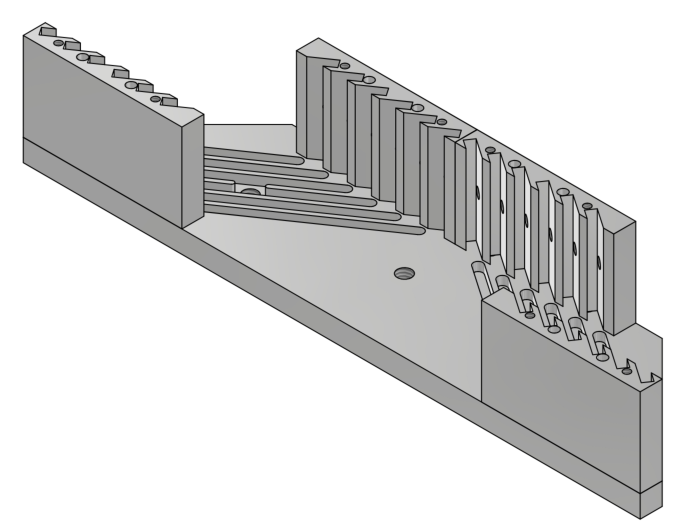
\includegraphics[width=\textwidth]{Figures/4_photonic_qubit_path/brewster_mount_3d.pdf}
		\caption{Isometric view.}
		\label{fig:brewster_mount_3d}
	\end{subfigure}

	\vspace{0.5em}

	\begin{subfigure}[b]{0.75\textwidth}
		\centering
		\includesvg[width=\textwidth]{Figures/4_photonic_qubit_path/brewster_mount_top_down.svg}
		\caption{Top-down view.}
		\label{fig:brewster_mount_top}
	\end{subfigure}
	\caption{Custom-machined mount for Brewster windows. The mount features two mirrored sections of angled slots, each holding up to six Brewster windows at $\sim\SI{55.48}{\degree}$.}
	\label{fig:brewster_mount}
\end{figure}

Furthermore, the Brewster window mount has two sections in which the layout of one half is mirrored to that of the other half. The reason being that each Brewster window laterally displaces the transmitted beam by a fixed amount due to refraction through the tilted plate. This significantly reduces the coupling into the cavity fiber. In order to combat this, the two halves of the mount are symmetrical to one another, so that the shift of the optical beam path on both sides cancel each other out. By reversing the tilt direction in the second half of the array, each displacement is compensated by the corresponding window in the mirrored section. Although this is only the case when the total amount of Brewster windows is even and both halves are balanced, at most the shift would be equal to that of a single Brewster window shifting the optical beam path. This can be compensated by realigning the input beam into the cavity fiber.\\

\section{Photon Qubit Input-Output Path}

For the atom-photon gate, weak coherent pulses are used in order to simulate the effect of single photons getting reflected from the cavity. It is therefore imperative to precisely control the power going into the cavity, and also the frequency of the light. For that specific task the following setup was constructed.

\begin{figure}[htbp]
	\centering
	\includesvg[inkscapelatex=false,width=0.65\textwidth]{Figures/4_photonic_qubit_path/aom_track.svg}
	\caption{Double-pass AOM setup on the AOM table.}
	\label{fig:setup_aom_table}
\end{figure}

Figure \ref{fig:setup_aom_table} showcases a double-pass AOM track. The light going into the AOM track, is blue detuned to the 2-1' transition of the $\text{D}_2\text{-line}$ by $\SI{480}{MHz}$. Part of the light (not shown here), can then be superimposed either with a stable reference frequency source like an optical frequency comb from the company \textit{MenloSystems GmbH} when the laser frequency does not need to be scanned, or with another laser, for when it does need to be scanned, e.g., for performing a normal-mode spectroscopy.
The polarization of the light first gets set by a $\lambda/2$ retardation waveplate (1) in order to pass through the polarizing beam splitter (2) in full transmission. A plano convex lens (3) focuses the light into an acousto-optic modulator (4).
In the double-pass configuration shown here, the AOM shifts the optical frequency by twice its driving frequency, enabling continuous frequency tuning.\\

The zeroth order of the transmitted light will get blocked by an iris, whereas the minus first order of the light is able to pass through. In order to now fully get reflected into the other arm of the PBS (marked in blue), the light passes through a $\lambda/4$ retardation plate (5) twice, while getting reflected and focused back into the AOM via a plano-concave mirror (6).

The light then passes through two sets of neutral density (ND) filters (7) (each set transmitting only $\simeq0.037\%$) and polarizers plus one $\lambda/2$ and $\lambda/4$ retardation waveplates (8) which allow for the alignment of the light with the principal axis of the polarization-maintaining (PM) fiber. The two sets of ND filters, can be selectively inserted into or removed from the beam path, attenuating the pulses to mean photon numbers in the range $\bar{n} = \{1\mathrm{e}{-5}, \ldots, 4\}$ at the cavity input, with both inserted. The light then gets sent to the atomic-table via another PM fiber.

\begin{figure}[htbp]
	\centering
	\makebox[\linewidth][c]{
		\includesvg[inkscapelatex=false,width=1.1\linewidth]{Figures/4_photonic_qubit_path/setup_w_detectors_no_aom.svg}
	}
	\caption{Optical setup on the atom-cavity table. The input photon is highlighted in red, and the reflected photon is highlighted in green.}
	\label{fig:setup_cavity_table}
\end{figure}

Once the light goes from the AOM table to the atom table, then the setup shown in Figure \ref{fig:setup_cavity_table} is used. The input polarization for the atom-photon gate is able to be set via two automatically controlled retardation waveplates (1), with the light coming from the AOM table. In order to compensate for the polarization-dependent losses the light then passes through the array of Brewster windows (2). A set of compensation waveplates (3) then ensure that the H and V polarized light interacting with the atom-cavity system, are mapped to the $\pi$ and $V$ eigenmodes of the cavity. In order to couple the light into the cavity fiber, it is reflected off of a pellicle beam splitter (6). The pellicle beam splitter reflects $1\%$ of the beam onto a mirror and through a dichroic mirror (4) into the cavity fiber coupler. The dichroic mirror also serves to couple the intracavity dipole trap light (not shown) into the same fiber. The light reflected from the birefringent cavity (5), passes through the dichroic mirror and reflects off the mirror back onto the pellicle. Since the pellicle transmits $\sim99\%$ of the returning light, the reflected signal continues with minimal loss (green path) to the detection stage. An arbitrary polarization measurement basis can then be set via two automatically controlled retardation waveplates (7). Finally the light passes through another PBS, and the two arms couple into two separate superconducting nanowire single-photon detectors (SNSPDs,8). The efficiency of the entire detection setup has an estimated $74.21\%$ at an average dark count rate of $\SI{43}{\hertz}$ per SNSPD channel. \\

Prior to building the setup shown in Figure \ref{fig:setup_cavity_table}, the gate photons were routed via an existing beam path known as the probe beam, which had originally been used for empty-cavity spectroscopy to determine the mode-matching efficiency and photon decay rate.

\begin{figure}[htbp]
	\centering
	\includesvg[inkscapelatex=false,width=\textwidth]{Figures/4_photonic_qubit_path/old_optical_path_setup_no_aom.svg}
	\caption{Old optical setup on the atom-cavity table. The input photon is highlighted in red, the reflected photon is highlighted in green, and the $\SI{772}{\nano\metre}$ short cavity trap ligth is highlighted in blue.}
	\label{fig:old_setup_cavity_table}
\end{figure}

The earlier setup can be seen in Figure \ref{fig:old_setup_cavity_table}. The light coming from the probe beam would be coupled into the cavity-fiber, through the transmission and subsequent reflection dichroic mirrors (4). Each of these mirrors is a \textit{LL01-785-12.5 MaxLine laser clean-up filter} from the company \textit{Semrock}, and possess the feature of transmitting most of the incoming light and reflecting only a small portion. This setup was chosen so that both the intracavity light trap (10) with its own set of compensation waveplates (7) and the probe beam, could be coupled into the fiber simultaneously.\\

The problem of this initial setup was, that precise control over the polarization and its losses is crucial, especially after reflection from the atom-cavity system. However, as it was the case with this setup, the coupling into the cavity fiber, was achieved via reflection off a dichroic mirror, which introduced additional polarization-dependent losses and rotations in the s and p polarization. In order to account for extra rotations induced by the dichroic mirrors (4), another set of compensation waveplates was included right in front of the cavity fiber coupler (5). This then meant that the first set of compensation waveplates (3), was meant to account for the rotations induced by the two dichroic mirrors, thus mapping the H and V polarization of the incoming light to the s and p polarization of the two mirrors. The second set of compensation waveplates (5) then mapped the s and p polarizations of the dichroic mirrors to the $\pi$ and V mode of the cavity. However, with no means to check the polarization of the reflected light from the dichroic mirror via a polarimeter, due to spatial constraints, this setup proved to be unreliable. The measurement setup with the automatic waveplates (8) and two SNSPDs (9) would have remained the same.\\

Finally, by changing to the setup shown in Figure \ref{fig:setup_cavity_table}, and instead opting to use a pellicle, which had much smaller polarization-dependent losses and rotations in reflection compared to the dichroic mirrors, this issue was resolved. Furthermore, it was verified that the polarization-dependent changes both in reflection and transmission through the pellicle were minimal, thus ensuring that the correctly reflected light will not receive further penalties when going to the detectors.

A quantitative comparison of the two configurations highlights the reduction of polarization-dependent losses when replacing the dichroic mirrors with a pellicle beam splitter. In the original setup, a pronounced imbalance between H and V polarizations is observed before the coupler, with relative transmission differences on the order of $\sim 20\text{--}30\%$, indicating significant polarization-dependent loss introduced by the dichroic elements. In contrast, for the pellicle-based configuration, the normalized transmissions for H and V are closely matched, corresponding to only a few fractions of a percent difference. This demonstrates that the pellicle substantially suppresses polarization-dependent losses compared to the old dichroic mirror configuration.
